%============================================================
% PharmaEase — Enterprise Software Requirements Specification
% Version 3.0 — MASSIVE EXPANSION EDITION
%============================================================

\documentclass[12pt,a4paper]{report}

%------------------------------------------------------------
% PACKAGES
%------------------------------------------------------------
\usepackage[T1]{fontenc}
\usepackage[utf8]{inputenc}
\usepackage{lmodern}
\usepackage[a4paper, margin=2.5cm, top=3cm, bottom=3cm]{geometry}
\usepackage{graphicx}
\usepackage{float}
\usepackage{booktabs}
\usepackage{longtable}
\usepackage{array}
\usepackage{tabularx}
\usepackage{multirow}
\usepackage{xcolor}
\usepackage{colortbl}
\usepackage[bookmarks=true, bookmarksnumbered=true, colorlinks=true]{hyperref}
\usepackage{enumitem}
\usepackage{fancyhdr}
\usepackage{titlesec}
\usepackage{tocloft}
\usepackage{setspace}
\usepackage{microtype}
\usepackage{caption}
\usepackage{subcaption}
\usepackage{amsmath}
\usepackage{amssymb}
\usepackage{listings}
\usepackage{mdframed}
\usepackage{makecell}
\usepackage{pifont}

%------------------------------------------------------------
% COLOUR PALETTE
%------------------------------------------------------------
\definecolor{pharmaBlue}{RGB}{26,82,118}
\definecolor{pharmaDark}{RGB}{15,50,80}
\definecolor{pharmaGreen}{RGB}{30,132,73}
\definecolor{pharmaGold}{RGB}{212,172,13}
\definecolor{pharmaRed}{RGB}{146,43,33}
\definecolor{pharmaGray}{RGB}{127,140,141}
\definecolor{lightBlue}{RGB}{213,234,246}
\definecolor{lightGreen}{RGB}{208,238,217}
\definecolor{lightOrange}{RGB}{255,230,200}
\definecolor{codeGray}{RGB}{248,248,248}
\definecolor{rowOdd}{RGB}{240,248,255}
\definecolor{rowEven}{RGB}{255,255,255}
\definecolor{headerBlue}{RGB}{26,82,118}

%------------------------------------------------------------
% HYPERREF SETUP
%------------------------------------------------------------
\hypersetup{
  linkcolor=pharmaBlue,
  citecolor=pharmaGreen,
  urlcolor=pharmaRed,
  pdftitle={PharmaEase — Enterprise SRS},
  pdfauthor={Wasif Ali, Anisa Khan},
}

%------------------------------------------------------------
% HEADER / FOOTER
%------------------------------------------------------------
\pagestyle{fancy}
\fancyhf{}
\fancyhead[L]{\small\color{pharmaGray}\textbf{PharmaEase}\ ---\ Enterprise SRS}
\fancyhead[R]{\small\color{pharmaGray}Air University Kamra}
\fancyfoot[L]{\small\color{pharmaGray}Wasif Ali (245187) $\cdot$ Anisa Khan (245215)}
\fancyfoot[C]{\small\color{pharmaGray}---\ \thepage\ ---}
\fancyfoot[R]{\small\color{pharmaGray}Version 3.0}
\renewcommand{\headrulewidth}{0.5pt}
\renewcommand{\footrulewidth}{0.5pt}

%------------------------------------------------------------
% CHAPTER / SECTION TITLES
%------------------------------------------------------------
\titleformat{\chapter}[block]
  {\normalfont\Huge\bfseries\color{pharmaBlue}}
  {\thechapter.}{0.5em}{}[{\color{pharmaGold}\titlerule[2pt]}]
\titlespacing{\chapter}{0pt}{-20pt}{20pt}

\titleformat{\section}
  {\normalfont\Large\bfseries\color{pharmaDark}}
  {\thesection}{0.8em}{}
\titlespacing{\section}{0pt}{16pt}{8pt}

\titleformat{\subsection}
  {\normalfont\large\bfseries\color{pharmaBlue}}
  {\thesubsection}{0.7em}{}
\titlespacing{\subsection}{0pt}{12pt}{6pt}

\titleformat{\subsubsection}
  {\normalfont\normalsize\bfseries\color{pharmaGreen}}
  {\thesubsubsection}{0.6em}{}

%------------------------------------------------------------
% CUSTOM ENVIRONMENTS
%------------------------------------------------------------
\newmdenv[
  linecolor=pharmaBlue, backgroundcolor=lightBlue!40, roundcorner=4pt,
  leftmargin=0pt, rightmargin=0pt, innerleftmargin=10pt, innerrightmargin=10pt,
  innertopmargin=10pt, innerbottommargin=10pt, linewidth=1.5pt,
]{infobox}

%------------------------------------------------------------
% CODE LISTING STYLE
%------------------------------------------------------------
\lstset{
  backgroundcolor=\color{codeGray}, basicstyle=\ttfamily\footnotesize,
  breaklines=true, frame=single, rulecolor=\color{pharmaGray},
  keywordstyle=\color{pharmaBlue}\bfseries, commentstyle=\color{pharmaGreen}\itshape,
  stringstyle=\color{pharmaRed}, numbers=left, numberstyle=\tiny\color{pharmaGray},
  numbersep=6pt, captionpos=b, tabsize=4, showstringspaces=false,
}

%------------------------------------------------------------
% SPACING (Set to 1.5 for academic reporting & padding)
%------------------------------------------------------------
\setstretch{1.5}
\setlength{\parskip}{10pt}
\setlength{\parindent}{0pt}
\captionsetup{font=small, labelfont={bf,color=pharmaBlue}, skip=8pt}

%============================================================
\begin{document}

%============================================================
%  BEAUTIFUL TITLE PAGE
%============================================================
\begin{titlepage}
\pagecolor{pharmaDark}
\color{white}
\centering
\vspace*{1cm}

% University Information
{\LARGE\bfseries\color{pharmaGold} AIR UNIVERSITY}\\[0.2cm]
{\Large DEPARTMENT OF COMPUTER SCIENCE}\\[0.1cm]
{\large AEROSPACE \& AVIATION CAMPUS, KAMRA}\\[0.8cm]
{\color{pharmaGold}\rule{14cm}{1.5pt}}\\[2.0cm]

% Project Title
{\fontsize{55}{65}\selectfont\bfseries PharmaEase}\\[0.5cm]
{\LARGE\itshape\color{pharmaGold} Enterprise Pharmacy Management System}\\[1.5cm]
{\color{pharmaGold}\rule{16cm}{3pt}}\\[1.5cm]

% Document Type
{\Huge\bfseries Software Requirements Specification}\\[0.4cm]

% Author Block (Better aligned with spacing)
\vspace{0.4cm}
\begin{center}
% move slightly to right
\hspace*{1cm}
\begin{tabular}{p{4cm} p{5cm}}
\multicolumn{1}{c}{
{\Large\bfseries Prepared By} }
\\[1cm]   % Gap below "Prepared By"
{\Large \textbf{Wasif Ali}} & {\Large \textit{Reg\#: 245187}}
\\[0.4cm] % Gap between authors
{\Large \textbf{Anisa Khan}} & {\Large \textit{Reg\#: 245215}}
\end{tabular}
\end{center}

\vfill
{\color{pharmaGold}\rule{12cm}{1pt}}\\[0.6cm]
{\large\itshape ``Connecting Patients to Medicines --- Reliably, Efficiently, Securely''}
\vspace*{1cm}
\end{titlepage}

\nopagecolor

%============================================================
%  ABSTRACT
%============================================================
\chapter*{Abstract}
\addcontentsline{toc}{chapter}{Abstract}

\textbf{PharmaEase} is an enterprise-grade, desktop-based Pharmacy Management System architected in \textbf{Java} and strictly governed by the \textbf{Model-View-Controller (MVC)} design paradigm. Supported by a highly normalized \textbf{MySQL} relational database backend, the system is designed to completely digitise, automate, and streamline core pharmacological workflows. By transitioning away from conventional paper-based ledgers, PharmaEase directly mitigates human error, improves inventory accuracy, guarantees secure data handling, and significantly enhances the operational efficiency of multi-seller pharmacy environments.

This Software Requirements Specification (SRS) is drafted in rigorous compliance with the \textbf{IEEE 830-1998 standard}. It provides an exhaustive decomposition of the software's constraints. It spans operational scope, in-depth functional and non-functional requirements, detailed use-case workflows, external interfaces, and advanced system modelling. The document incorporates high-fidelity UML artefacts—including Architecture, Use Case, Activity, Sequence, Class, Domain, and Entity-Relationship Diagrams. All documentation has been reverse-engineered directly from the final Java codebase to guarantee absolute structural parity between the written blueprint and the deployed software product.

\vspace{1em}
\begin{infobox}
\textbf{Executive Summary:}
This document serves as the absolute source of truth for the PharmaEase project. It details the secure authentication protocols, multi-threaded inventory handling mechanisms, and strict role-based access controls designed, developed, and tested by Wasif Ali and Anisa Khan at Air University, Kamra.
\end{infobox}

\clearpage

%============================================================
\tableofcontents
\listoffigures
\clearpage

%============================================================
%  CHAPTER 1: INTRODUCTION
%============================================================
\chapter{Introduction}

\section{Purpose}
The purpose of this document is to formally specify the software requirements for \textbf{PharmaEase}, a comprehensive Pharmacy Management System (PMS). It serves as a binding contract between the development team and the project stakeholders (academic supervisors). This SRS guarantees that developers, database administrators, and software testers possess a unified, unambiguous understanding of the software's capabilities, technical constraints, and operational environment before final evaluation.

\section{Document Scope and Organization}
This SRS systematically details the complete lifecycle requirements of the PharmaEase application. 
\begin{itemize}
    \item \textbf{Chapters 1 \& 2:} Define the business context, regulatory requirements, user profiles, and operational boundaries of the software.
    \item \textbf{Chapter 3:} Provides an exhaustive breakdown of the functional requirements, formatted as testable Use Case narratives.
    \item \textbf{Chapter 4:} Details the Data Dictionary, outlining every database table, column, and relationship.
    \item \textbf{Chapter 5 \& 6:} Outline non-functional requirements (security, performance) and system interfaces.
    \item \textbf{Chapter 7:} Presents the structural and behavioral UML diagrams that map the system's architecture.
    \item \textbf{Chapter 8 \& 9:} Dictate the testing strategies, test cases, and the Requirements Traceability Matrix (RTM).
\end{itemize}

\section{Product Scope and Business Context}
PharmaEase is conceived as a \textbf{standalone, multi-role desktop application} operating on a local area network (LAN) or single-machine environment. The primary business objective is to eliminate the inefficiencies, stock miscalculations, and security risks associated with manual pharmacy bookkeeping.

The software systematically handles three distinct operational domains:
\begin{enumerate}
    \item \textbf{Administrative Domain:} Offers system-wide oversight. Administrators possess global management privileges to curate the central medicine catalog, categorize pharmaceuticals, audit user accounts, and review aggregate financial metrics.
    \item \textbf{Seller Domain:} Provides certified pharmacists with an isolated Point-of-Sale (POS) and inventory management interface. Sellers track specific medical batches, monitor expiry dates, and process customer orders dynamically without interfering with system-level configurations.
    \item \textbf{Customer Domain:} Delivers an intuitive storefront. End-users can securely browse the medical catalog, manage a persistent shopping cart, execute checkouts, and submit digital prescriptions required for restricted or controlled substances.
\end{enumerate}

\section{Definitions, Acronyms, and Abbreviations}
\begin{longtable}{>{\bfseries}p{3.5cm} p{11cm}}
\toprule
\rowcolor{headerBlue}\color{white}\textbf{Term} & \color{white}\textbf{Definition} \\
\midrule
\endfirsthead
\rowcolor{rowOdd}  MVC          & Model-View-Controller: An architectural pattern separating UI (View), logic (Controller), and data (Model). \\
\rowcolor{rowEven} JDBC         & Java Database Connectivity: The standard Java API for establishing connections to relational databases. \\
\rowcolor{rowOdd}  RBAC         & Role-Based Access Control: A security paradigm restricting system access based on the logged-in user's role. \\
\rowcolor{rowEven} POJO         & Plain Old Java Object: Pure data structures used in the Model layer, containing private fields and public getters/setters. \\
\rowcolor{rowOdd}  CRUD         & Create, Read, Update, Delete: The four fundamental operations of persistent storage. \\
\rowcolor{rowEven} ERD          & Entity-Relationship Diagram: A visual representation of the database schema and foreign key relationships. \\
\rowcolor{rowOdd}  RTM          & Requirements Traceability Matrix: A document mapping functional requirements to specific test cases. \\
\rowcolor{rowEven} GUI          & Graphical User Interface: The visual components (Java Swing) the user interacts with. \\
\rowcolor{rowOdd}  SQL Injection & A code injection technique that might destroy a database; prevented in this project via \texttt{PreparedStatements}. \\
\bottomrule
\end{longtable}

\section{References}
\begin{enumerate}
    \item IEEE Computer Society. (1998). \textit{IEEE Recommended Practice for Software Requirements Specifications} (IEEE Std 830-1998).
    \item Gamma, E., Helm, R., Johnson, R., \& Vlissides, J. (1994). \textit{Design Patterns: Elements of Reusable Object-Oriented Software}. Addison-Wesley.
    \item Oracle Corporation. (2023). \textit{Java Platform, Standard Edition 17 API Specification}.
    \item MySQL AB. (2023). \textit{MySQL 8.0 Reference Manual}.
\end{enumerate}

\clearpage

%============================================================
%  CHAPTER 2: OVERALL DESCRIPTION
%============================================================
\chapter{Overall Description}

\section{Product Perspective}
PharmaEase operates as an independent, self-contained desktop system. However, its architecture simulates a highly scalable enterprise environment by strictly isolating the Java Swing Graphical User Interface (GUI) from the MySQL persistence layer. The \texttt{DBConnection} class utilizes the Singleton design pattern to ensure optimal network resource management, mitigating the risk of database lockouts, memory leaks, and connection pool exhaustion during simultaneous multi-user transactions.

\section{User Classes and Characteristics (Personas)}
To maintain strict data security and operational integrity, the system divides user access into three rigid, mutually exclusive tiers.

\subsection{Administrator (Super User)}
\begin{itemize}
    \item \textbf{Technical Expertise:} High. Understands database concepts and system management.
    \item \textbf{Privileges:} Unrestricted CRUD access to global tables (Users, Medicines, Categories).
    \item \textbf{Responsibilities:} The Admin is responsible for onboarding new medicines into the global catalog to prevent data duplication. They monitor system health, oversee seller activities, and handle user dispute resolutions.
\end{itemize}

\subsection{Seller / Pharmacist (Standard User)}
\begin{itemize}
    \item \textbf{Technical Expertise:} Medium. Comfortable with standard Point-of-Sale (POS) systems.
    \item \textbf{Privileges:} Confined entirely to inventory management and order processing for their specific assigned ID.
    \item \textbf{Responsibilities:} Adding physical stock batches to the database, ensuring expiry dates are accurately logged, and processing incoming orders routed to their pharmacy.
\end{itemize}

\subsection{Customer (End User)}
\begin{itemize}
    \item \textbf{Technical Expertise:} Low to Medium. Requires a highly intuitive, visually guided interface.
    \item \textbf{Privileges:} Can only view the global catalog, place personal orders, and view their own purchase history.
    \item \textbf{Responsibilities:} Searching for medicines, maintaining their shopping cart, uploading valid prescriptions for controlled substances, and executing secure checkouts.
\end{itemize}

\section{Operating Environment}
The software is designed to be highly portable across modern operating systems.
\begin{itemize}
    \item \textbf{Client Platform:} Java Runtime Environment (JRE) Version 17 or higher. Fully cross-platform (Windows 10/11, macOS 12+, Linux Ubuntu 20.04+).
    \item \textbf{Database Server:} MySQL Community Server Version 8.0 or higher.
    \item \textbf{Development IDE:} Eclipse IDE for Enterprise Java.
    \item \textbf{Hardware Minimums:} 4GB RAM, Intel Core i3 Processor (or AMD equivalent), 500MB available disk space, $1280 \times 720$ minimum display resolution.
\end{itemize}

\section{Design and Implementation Constraints}
\begin{itemize}
    \item \textbf{UI Limitations:} Java Swing relies on absolute (\texttt{null}) layouts in this specific application to ensure pixel-perfect rendering of the complex dashboard elements. Consequently, dynamic window resizing is disabled to prevent UI component overlapping.
    \item \textbf{Database Dependency:} The application is purely a client; it cannot operate offline. A persistent TCP/IP connection to the localhost (or remote) MySQL instance is mandatory for all operations.
    \item \textbf{Storage Limitations:} Prescriptions are currently handled via textual input (Doctor Name, Date, Notes) rather than physical image/PDF uploads due to BLOB storage constraints in the current prototype phase.
\end{itemize}

\section{Assumptions and Dependencies}
\begin{enumerate}
    \item It is assumed that the host machine running the software has the MySQL service actively running on default port 3306.
    \item It is assumed that the \texttt{mysql-connector-java-8.x.jar} driver is correctly configured in the Java Build Path.
    \item It is assumed that the database schema (\texttt{pharmacy\_management.sql}) has been successfully imported and executed prior to launching the \texttt{PharmaEase.java} entry point.
    \item At least one default Administrator account must be hard-coded or manually inserted into the database to allow initial system configuration.
\end{enumerate}

\clearpage

%============================================================
%  CHAPTER 3: DETAILED FUNCTIONAL REQUIREMENTS
%============================================================
\chapter{Detailed Functional Requirements}

This section outlines the precise, testable functional requirements of the PharmaEase system. They are structured as detailed Use Case specifications to provide absolute clarity to the development and testing teams.

\section{FR Group 1: User Management \& Authentication}

\subsection{FR 1.1: Multi-Role Account Registration}
\begin{itemize}
    \item \textbf{Description:} The system shall provide a unified graphical interface for new users to register as either a Customer or a Seller.
    \item \textbf{Pre-conditions:} The MySQL database is active, and the \texttt{users} table is accessible.
    \item \textbf{Normal Flow:}
        \begin{enumerate}
            \item User selects "Sign Up" from the main splash screen.
            \item User enters standard details: Username, Password, Email, Phone, Address.
            \item User selects their desired Role (Customer or Seller) via a dropdown or radio button.
            \item If "Seller" is selected, the GUI dynamically reveals additional mandatory fields: "Pharmacy Name" and "License Number".
            \item User clicks Submit.
            \item The \texttt{UserController} verifies that the chosen Username does not already exist.
            \item System executes an \texttt{INSERT} into the core \texttt{users} table, retrieves the generated \texttt{user\_id}, and executes a secondary \texttt{INSERT} into the specific role table (\texttt{customers} or \texttt{sellers}).
        \end{enumerate}
    \item \textbf{Alternative Flow:} If the Username exists, a \texttt{JOptionPane} error is displayed, and the process halts.
    \item \textbf{Post-conditions:} A new user record is permanently established in the database.
\end{itemize}

\subsection{FR 1.2: Secure Login and Role Dispatch}
\begin{itemize}
    \item \textbf{Description:} The system must authenticate credentials and route the user to their specific, restricted dashboard.
    \item \textbf{Normal Flow:}
        \begin{enumerate}
            \item User inputs Username and Password.
            \item \texttt{UserController.validateLogin()} executes a \texttt{PreparedStatement} querying the database.
            \item If credentials match, the system retrieves the \texttt{user\_type\_id}.
            \item The current \texttt{LoginPage} \texttt{JFrame} is disposed of.
            \item Based on the ID, the system instantiates either \texttt{AdminDashboard}, \texttt{SellerDashboard}, or \texttt{CustomerDashboard}.
        \end{enumerate}
    \item \textbf{Post-conditions:} A secure session is initiated within the bounds of the user's RBAC privileges.
\end{itemize}

\section{FR Group 2: Medicine \& Inventory Operations}

\subsection{FR 2.1: Global Medicine Catalog Management}
\begin{itemize}
    \item \textbf{Description:} Administrators alone possess the right to define new medicines in the system to prevent Sellers from creating duplicate, conflicting records of the same drug.
    \item \textbf{Pre-conditions:} User is authenticated as an Admin.
    \item \textbf{Normal Flow:}
        \begin{enumerate}
            \item Admin accesses the "Manage Medicines" tab.
            \item Admin inputs Name, Manufacturer, Price, Category ID, and toggles the \texttt{RequiresPrescription} boolean flag.
            \item System validates inputs (e.g., Price $> 0$).
            \item System performs \texttt{INSERT INTO medicines}.
        \end{enumerate}
    \item \textbf{Post-conditions:} The new medicine immediately populates in the search grids for all Customers and Sellers globally.
\end{itemize}

\subsection{FR 2.2: Batch-Level Inventory Tracking}
\begin{itemize}
    \item \textbf{Description:} Sellers must add physical stock to the system. Stock is tracked by unique batch numbers to monitor expirations.
    \item \textbf{Normal Flow:}
        \begin{enumerate}
            \item Seller selects a globally defined Medicine from the catalog.
            \item Seller inputs a unique Batch Number, Quantity received, Manufacturing Date, and Expiry Date.
            \item System ensures the Expiry Date is chronologically after the Manufacturing Date and current system date.
            \item System executes \texttt{INSERT INTO inventory}.
        \end{enumerate}
    \item \textbf{Post-conditions:} The specific Seller's inventory is increased. Customers can now purchase this medicine.
\end{itemize}

\section{FR Group 3: Order Processing \& Checkout}

\subsection{FR 3.1: Persistent Shopping Cart Operations}
\begin{itemize}
    \item \textbf{Description:} Customers must be able to browse available inventory and build a prospective order.
    \item \textbf{Normal Flow:}
        \begin{enumerate}
            \item Customer views available medicines in a \texttt{JTable}.
            \item Customer selects an item, enters a quantity, and clicks "Add to Cart".
            \item System verifies that the requested quantity is $\leq$ the total available stock in the \texttt{inventory} table.
            \item The item is added to the in-memory cart, and the sub-total and grand total fields are dynamically updated.
        \end{enumerate}
\end{itemize}

\subsection{FR 3.2: Transactional Order Placement}
\begin{itemize}
    \item \textbf{Description:} The checkout mechanism must be atomic and fail-safe to prevent database corruption.
    \item \textbf{Normal Flow:}
        \begin{enumerate}
            \item Customer initiates Checkout.
            \item System invokes \texttt{java.sql.Connection.setAutoCommit(false)} to begin a transaction block.
            \item System creates the header record: \texttt{INSERT INTO orders}.
            \item System loops through cart items, executing \texttt{INSERT INTO order\_items}.
            \item System executes \texttt{UPDATE inventory SET quantity = quantity - requested\_qty}.
            \item If all steps succeed, \texttt{Connection.commit()} is executed.
        \end{enumerate}
    \item \textbf{Exception Flow:} If a SQL error occurs (e.g., another user bought the last item milliseconds prior), an \texttt{SQLException} is caught, \texttt{Connection.rollback()} is executed, and the user is notified.
\end{itemize}

\subsection{FR 3.3: Legal Prescription Validation}
\begin{itemize}
    \item \textbf{Description:} The system must legally restrict the sale of controlled substances unless an authorisation record exists.
    \item \textbf{Normal Flow:}
        \begin{enumerate}
            \item During checkout initiation, the system iterates over the cart.
            \item If any \texttt{Medicine} object has \texttt{requires\_prescription == 1}, checkout is paused.
            \item A modal window forces the Customer to input prescription details (Doctor Name, Issue Date).
            \item These details are inserted into the \texttt{prescriptions} table.
            \item The newly generated \texttt{prescription\_id} is retrieved and permanently linked as a Foreign Key to the \texttt{orders} table during final placement.
        \end{enumerate}
\end{itemize}

\clearpage

%============================================================
%  CHAPTER 4: DATA DICTIONARY & DATABASE DESIGN
%============================================================
\chapter{Data Dictionary}

The PharmaEase system relies on a highly normalized MySQL database structure. This data dictionary explicitly defines the purpose, data type, and constraints of every critical field in the core tables.

\section{Table: \texttt{users}}
Central repository for all system authentication and baseline contact information.
\begin{longtable}{>{\ttfamily}p{3cm} p{3cm} p{2cm} p{6cm}}
\toprule
\rowcolor{headerBlue}\color{white}\textbf{Column Name} & \color{white}\textbf{Data Type} & \color{white}\textbf{Keys} & \color{white}\textbf{Description} \\
\midrule
\endfirsthead
user\_id & INT & PK & Auto-incrementing unique identifier. \\
\rowcolor{rowOdd}username & VARCHAR(100)& UNIQUE & Login identifier; must be unique system-wide. \\
password & VARCHAR(255)& NN & User password. \\
\rowcolor{rowOdd}email & VARCHAR(150)& & User's contact email. \\
user\_type\_id & INT & FK, NN & Links to \texttt{user\_type} table (1=Admin, 2=Seller, 3=Customer). \\
\rowcolor{rowOdd}created\_at & TIMESTAMP & & Automatically generated timestamp of account creation. \\
\bottomrule
\end{longtable}

\section{Table: \texttt{medicines}}
The global catalog of all pharmaceutical items, managed exclusively by Administrators.
\begin{longtable}{>{\ttfamily}p{4.5cm} p{2.8cm} p{2cm} p{5cm}}
\toprule
\rowcolor{headerBlue}\color{white}\textbf{Column Name} & \color{white}\textbf{Data Type} & \color{white}\textbf{Keys} & \color{white}\textbf{Description} \\
\midrule
\endfirsthead
medicine\_id & INT & PK & Auto-incrementing identifier. \\
\rowcolor{rowOdd}name & VARCHAR(150)& NN & Commercial or generic name of the drug. \\
manufacturer & VARCHAR(150)& & The company producing the drug. \\
\rowcolor{rowOdd}category\_id & INT & FK & Links to the \texttt{categories} taxonomy table. \\
requires\_prescription & BOOLEAN & NN & 1 (True) blocks sale without an Rx; 0 (False) allows OTC sale. \\
\rowcolor{rowOdd}unit\_price & DECIMAL & NN & Standardized global pricing for the item. \\
\bottomrule
\end{longtable}

\section{Table: \texttt{inventory}}
Tracks physical stock at the batch level, linked to specific sellers.
\begin{longtable}{>{\ttfamily}p{3cm} p{3cm} p{2cm} p{6cm}}
\toprule
\rowcolor{headerBlue}\color{white}\textbf{Column Name} & \color{white}\textbf{Data Type} & \color{white}\textbf{Keys} & \color{white}\textbf{Description} \\
\midrule
\endfirsthead
inventory\_id & INT & PK & Auto-increment identifier. \\
\rowcolor{rowOdd}medicine\_id & INT & FK, NN & Links to the global \texttt{medicines} catalog. \\
seller\_id & INT & FK, NN & The specific pharmacist holding this stock. \\
\rowcolor{rowOdd}batch\_number & VARCHAR(100)& UNIQUE & Manufacturer's specific batch lot number. \\
quantity & INT & NN & Current available stock level. Decrements on sale. \\
\rowcolor{rowOdd}expiry\_date & DATE & NN & Critical date for expiration alerts in seller dashboard. \\
\bottomrule
\end{longtable}

\section{Table: \texttt{orders} and \texttt{order\_items}}
Handles the financial and transactional records.
\begin{longtable}{>{\ttfamily}p{3.5cm} p{2cm} p{2cm} p{6.5cm}}
\toprule
\rowcolor{headerBlue}\color{white}\textbf{Column Name} & \color{white}\textbf{Data Type} & \color{white}\textbf{Keys} & \color{white}\textbf{Description} \\
\midrule
\endfirsthead
order\_id & INT & PK & Header ID for the entire purchase. \\
\rowcolor{rowOdd}customer\_id & INT & FK, NN & The user who placed the order. \\
total\_amount & DECIMAL & NN & Sum of all sub-totals in the cart. \\
\rowcolor{rowOdd}prescription\_id & INT & FK & Nullable. Linked if restricted items were purchased. \\
\midrule
item\_id & INT & PK & Individual line item ID. \\
\rowcolor{rowOdd}order\_id & INT & FK, NN & Link back to the parent order header. \\
inventory\_id & INT & FK, NN & Exact batch the item was deducted from. \\
\rowcolor{rowOdd}subtotal & DECIMAL & NN & Quantity multiplied by Unit Price. \\
\bottomrule
\end{longtable}

\clearpage

%============================================================
%  CHAPTER 5: NON-FUNCTIONAL REQUIREMENTS
%============================================================
\chapter{Non-Functional Requirements}

\section{Performance \& Scalability Metrics}
\begin{itemize}
    \item \textbf{NFR-01 [Query Latency]:} Under normal local network loads, any CRUD operation (e.g., retrieving the medicine catalog or submitting an order) must complete database interaction and render the updated UI state in \textbf{less than 2.0 seconds}.
    \item \textbf{NFR-02 [Concurrent Locking]:} The system must safely handle simultaneous inventory updates. If Customer A and Customer B attempt to purchase the same inventory batch simultaneously, the MySQL database's implicit row-level locking during the JDBC transaction must ensure stock is never drawn below zero.
    \item \textbf{NFR-03 [Memory Management]:} The application footprint should not exceed 500MB of RAM during peak usage to ensure it can run on legacy pharmacy terminal hardware.
\end{itemize}

\section{Security \& Access Control}
\begin{itemize}
    \item \textbf{NFR-04 [Role Isolation]:} Strict Role-Based Access Control (RBAC) must be enforced at the memory and controller level. The system architecture must programmatically prevent a Customer instance from instantiating a \texttt{SellerDashboard} or \texttt{AdminDashboard} object, regardless of UI manipulation.
    \item \textbf{NFR-05 [SQL Injection Prevention]:} Absolute prohibition of concatenated SQL query strings. Every single database interaction must utilize Java's \texttt{PreparedStatement} interface to rigorously sanitize user inputs and eliminate SQL injection attack vectors.
\end{itemize}

\section{Reliability and Robustness}
\begin{itemize}
    \item \textbf{NFR-06 [Graceful Degradation]:} The system must include comprehensive \texttt{try-catch} exception handling blocks for all \texttt{SQLExceptions}. If the MySQL server goes offline, the application must not crash to the desktop; instead, it must display a modal \texttt{JOptionPane} advising the user to check network connectivity.
    \item \textbf{NFR-07 [Atomicity]:} Financial and inventory transactions must adhere to ACID properties. A failure at any point in the checkout loop must trigger an automatic \texttt{Connection.rollback()} to maintain database integrity.
\end{itemize}

\section{Maintainability and Code Quality}
\begin{itemize}
    \item \textbf{NFR-08 [MVC Strictness]:} The architecture must guarantee that changes made to the Swing UI (e.g., changing a button color or moving a table) require absolutely zero modifications to the underlying SQL query strings in the Controller classes.
    \item \textbf{NFR-09 [Code Convention]:} All Java code must follow standard Oracle naming conventions (CamelCase for variables/methods, PascalCase for classes) and contain detailed Javadoc comments for all public Controller methods.
\end{itemize}

\clearpage

%============================================================
%  CHAPTER 6: SYSTEM INTERFACES
%============================================================
\chapter{System Interfaces}

\section{User Interfaces (UI)}
The Graphical User Interface is developed entirely using the core Java Swing toolkit (\texttt{javax.swing.*}) and AWT (\texttt{java.awt.*}).
\begin{itemize}
    \item \textbf{Layout Methodology:} The system utilizes Absolute Positioning (\texttt{setLayout(null)}) to allow precise pixel-level placement of complex dashboard elements, overriding default layout managers.
    \item \textbf{Visual Consistency:} A unified corporate color palette (PharmaBlue, White, Light Gray) is applied via custom \texttt{BackgroundPanel} classes.
    \item \textbf{User Feedback:} The UI relies heavily on \texttt{JTable} for data display. Custom \texttt{ButtonEditor} and \texttt{ButtonRenderer} classes are injected into table cells to allow users to interact with individual rows (e.g., clicking "Add to Cart" directly inside a table cell).
\end{itemize}

\section{Software Interfaces}
\begin{itemize}
    \item \textbf{Database Management System:} MySQL Community Edition 8.0.
    \item \textbf{Communication Protocol:} Java Database Connectivity (JDBC) API.
    \item \textbf{Driver:} \texttt{mysql-connector-java.jar} acts as the software bridge translating Java method calls into MySQL-compatible TCP/IP packets.
\end{itemize}

\section{Hardware Interfaces}
The application requires no specialized medical or pharmacy hardware (e.g., barcode scanners or specialized receipt printers are currently out of scope). It interacts with standard HID peripherals (mouse, keyboard) and utilizes the OS's default print spooler for generating PDF bills.

\clearpage

%============================================================
%  CHAPTER 7: SYSTEM MODELING & DIAGRAMS
%============================================================
\chapter{System Modeling and Diagrams}

To guarantee strict alignment between this specification document and the physical software, the following UML diagrams have been reverse-engineered from the final Java implementation. 

\section{System Architecture Diagram}
\begin{figure}[H]
    \centering
    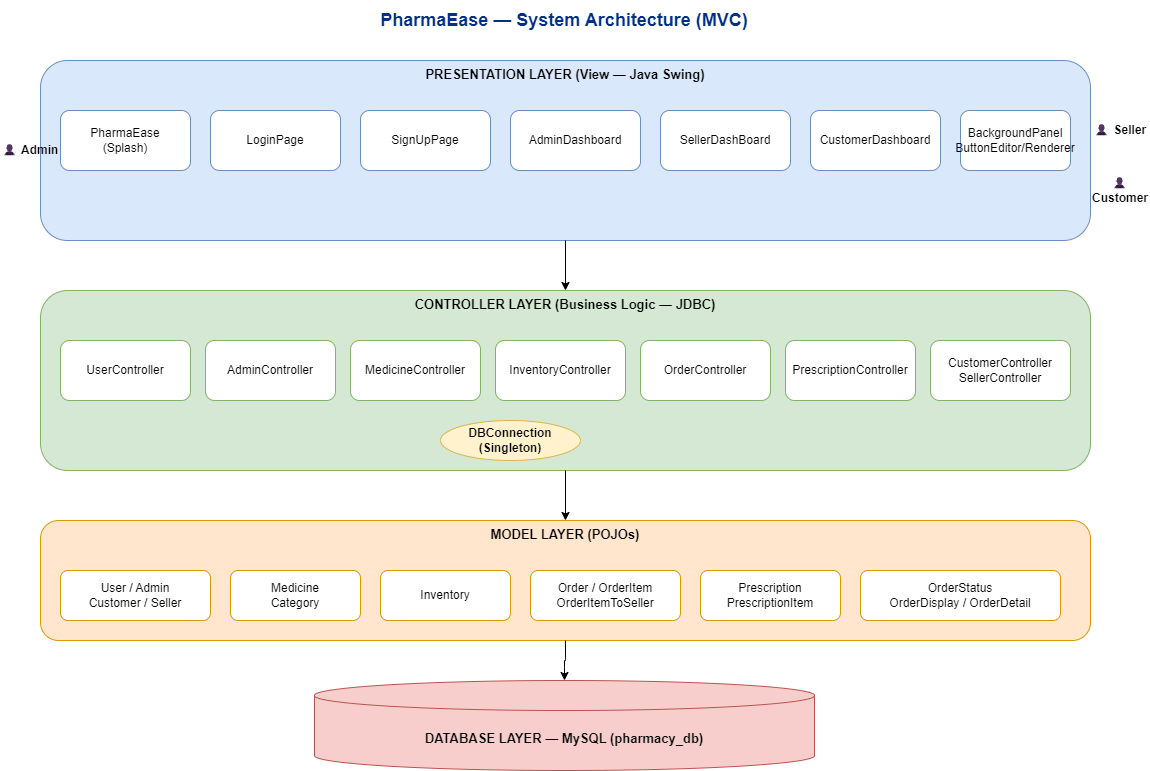
\includegraphics[width=\textwidth]{01_Architecture_Diagram.drawio.png}
    \caption{Three-Tier System Architecture (MVC Pattern)}
    \label{fig:architecture}
\end{figure}
PharmaEase implements a rigid \textbf{3-Tier MVC Architecture}. 
\begin{itemize}
    \item \textbf{View Layer (Swing):} Captures input and renders data. It has no knowledge of SQL.
    \item \textbf{Controller Layer:} The intermediary that receives UI events, processes business logic, and instantiates the \texttt{DBConnection} Singleton to talk to the database.
    \item \textbf{Model/Database Layer:} Defines the structure of the data via Java POJOs and persists it via MySQL.
\end{itemize}



\section{Use Case Diagram}
The Use Case Diagram defines the operational boundaries of the system. It maps the distinct functional permissions granted to the Admin, Seller, and Customer actors, clearly delineating the separation of concerns within the software.

\begin{figure}[H]
    \centering
    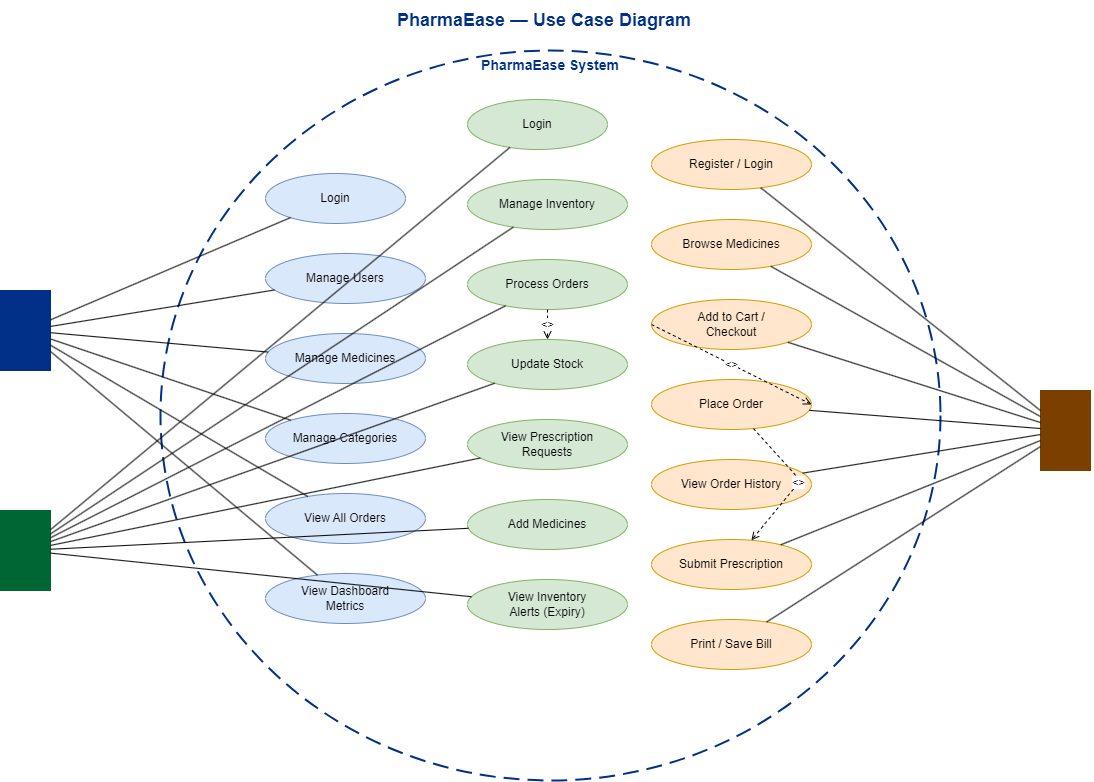
\includegraphics[width=0.95\textwidth]{02_UseCase_Diagram.drawio.png}
    \caption{PharmaEase System Use Case Diagram}
    \label{fig:usecase}
\end{figure}

\clearpage

\section{Domain Model}
This conceptual model abstracts the real-world pharmacy environment into software entities. It visually describes the cardinality and relationships between Users, Orders, Inventory Batches, and Prescriptions.

\begin{figure}[H]
    \centering
    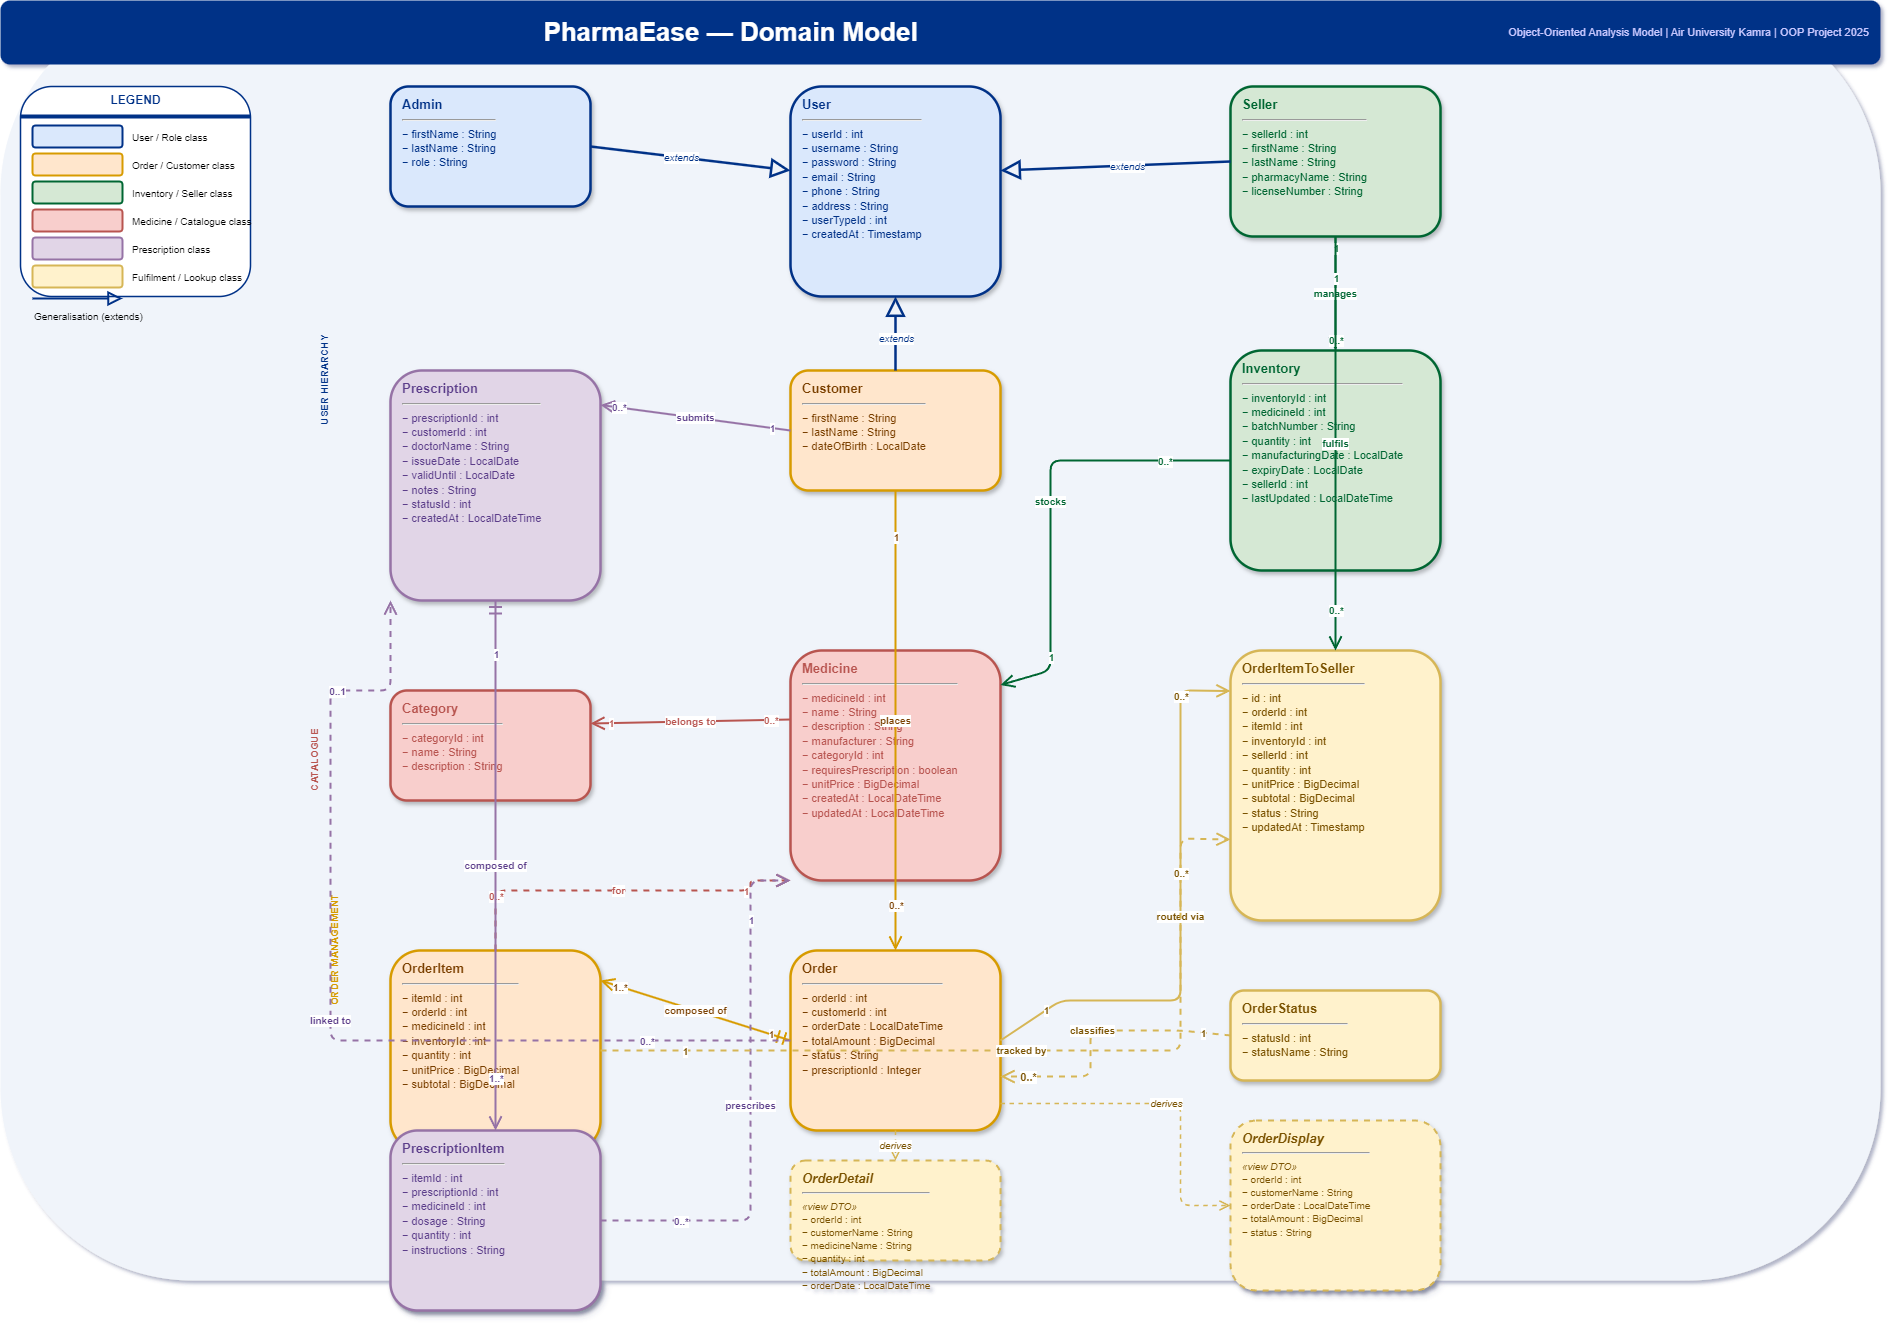
\includegraphics[width=0.9\textwidth]{PharmaEase_Domain_Model.drawio.png}
    \caption{PharmaEase Conceptual Domain Model}
    \label{fig:domain}
\end{figure}

\clearpage

\section{Activity and Class Diagrams}
The \textbf{Activity Diagram} tracks the complex flow of control across swim-lanes (Customer, System Controller, Seller) during a checkout process. The \textbf{Class Diagram} maps the exact static structure of the Java POJOs, displaying attributes, methods, and inheritance paths.

\begin{figure}[H]
    \centering
    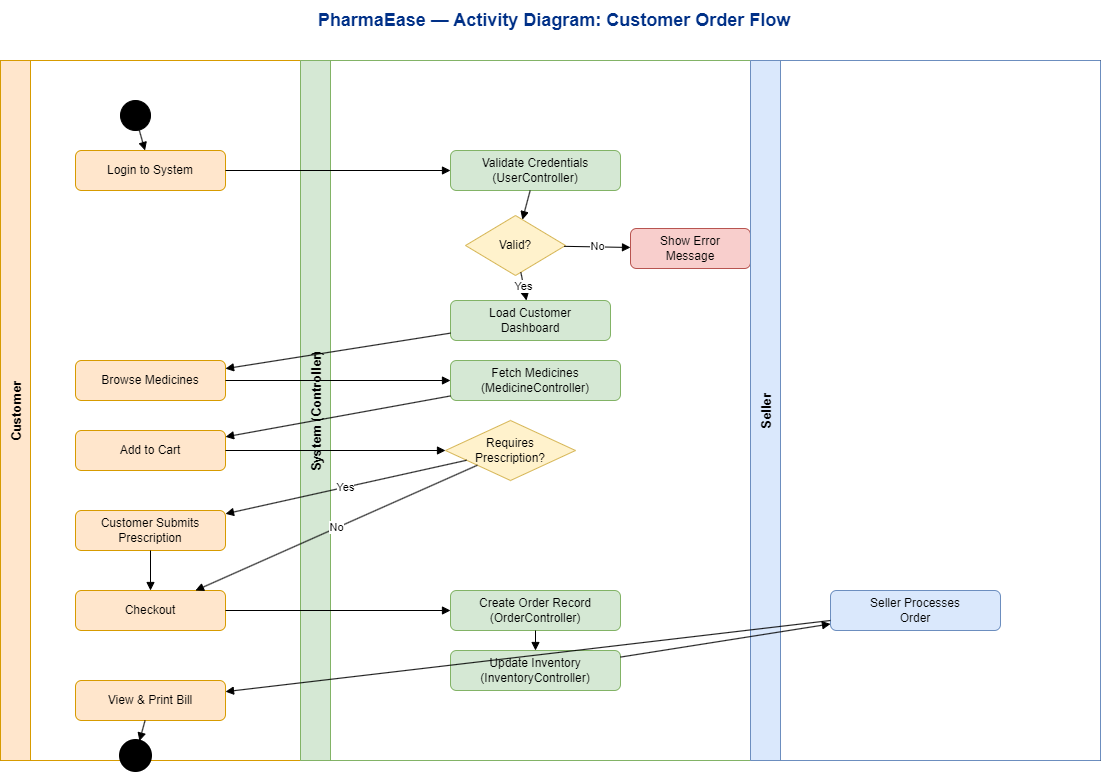
\includegraphics[width=\textwidth]{04_Activity_and_ClassDiagram.png}
    \caption{Activity Workflow and Static Class Structure}
    \label{fig:activity_class}
\end{figure}

\clearpage

\section{Sequence Diagram}
The Sequence Diagram models dynamic object interaction over time. It traces the exact chronological path of method invocations triggered by a user clicking a button on the UI layer, traveling through the \texttt{OrderController}, down to the \texttt{DBConnection}, executing the SQL, and returning the generated Order ID back up the stack.

\begin{figure}[H]
    \centering
    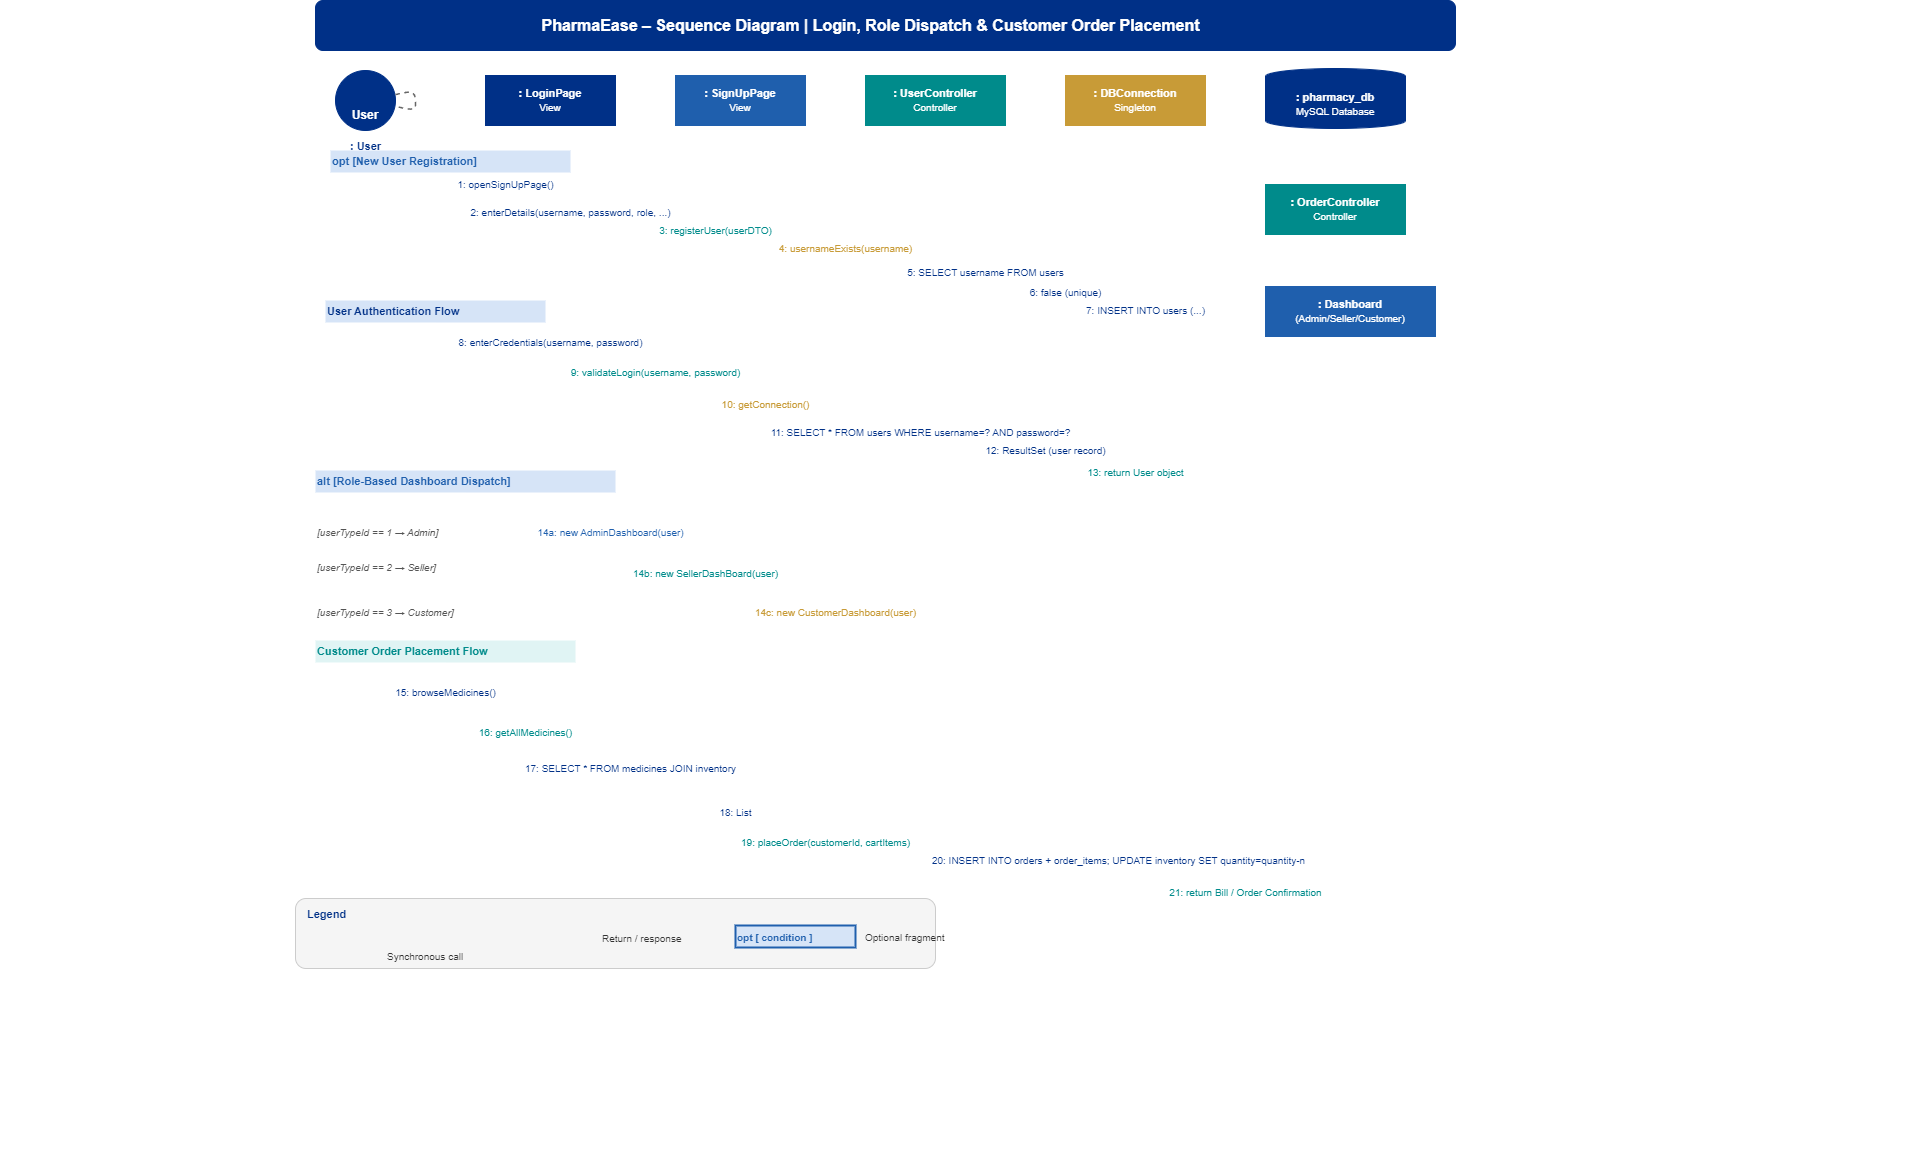
\includegraphics[width=\textwidth]{05_Sequence_Diagram.drawio.png}
    \caption{System Sequence Diagram (Authentication \& Checkout Flow)}
    \label{fig:sequence}
\end{figure}

\clearpage

\section{Entity-Relationship Diagram (ERD)}
The MySQL database is highly normalized (Third Normal Form) to ensure zero data redundancy. This ERD illustrates the primary keys (PK), foreign keys (FK), and multiplicity constraints governing the 14 core tables in the backend.

\begin{figure}[H]
    \centering
    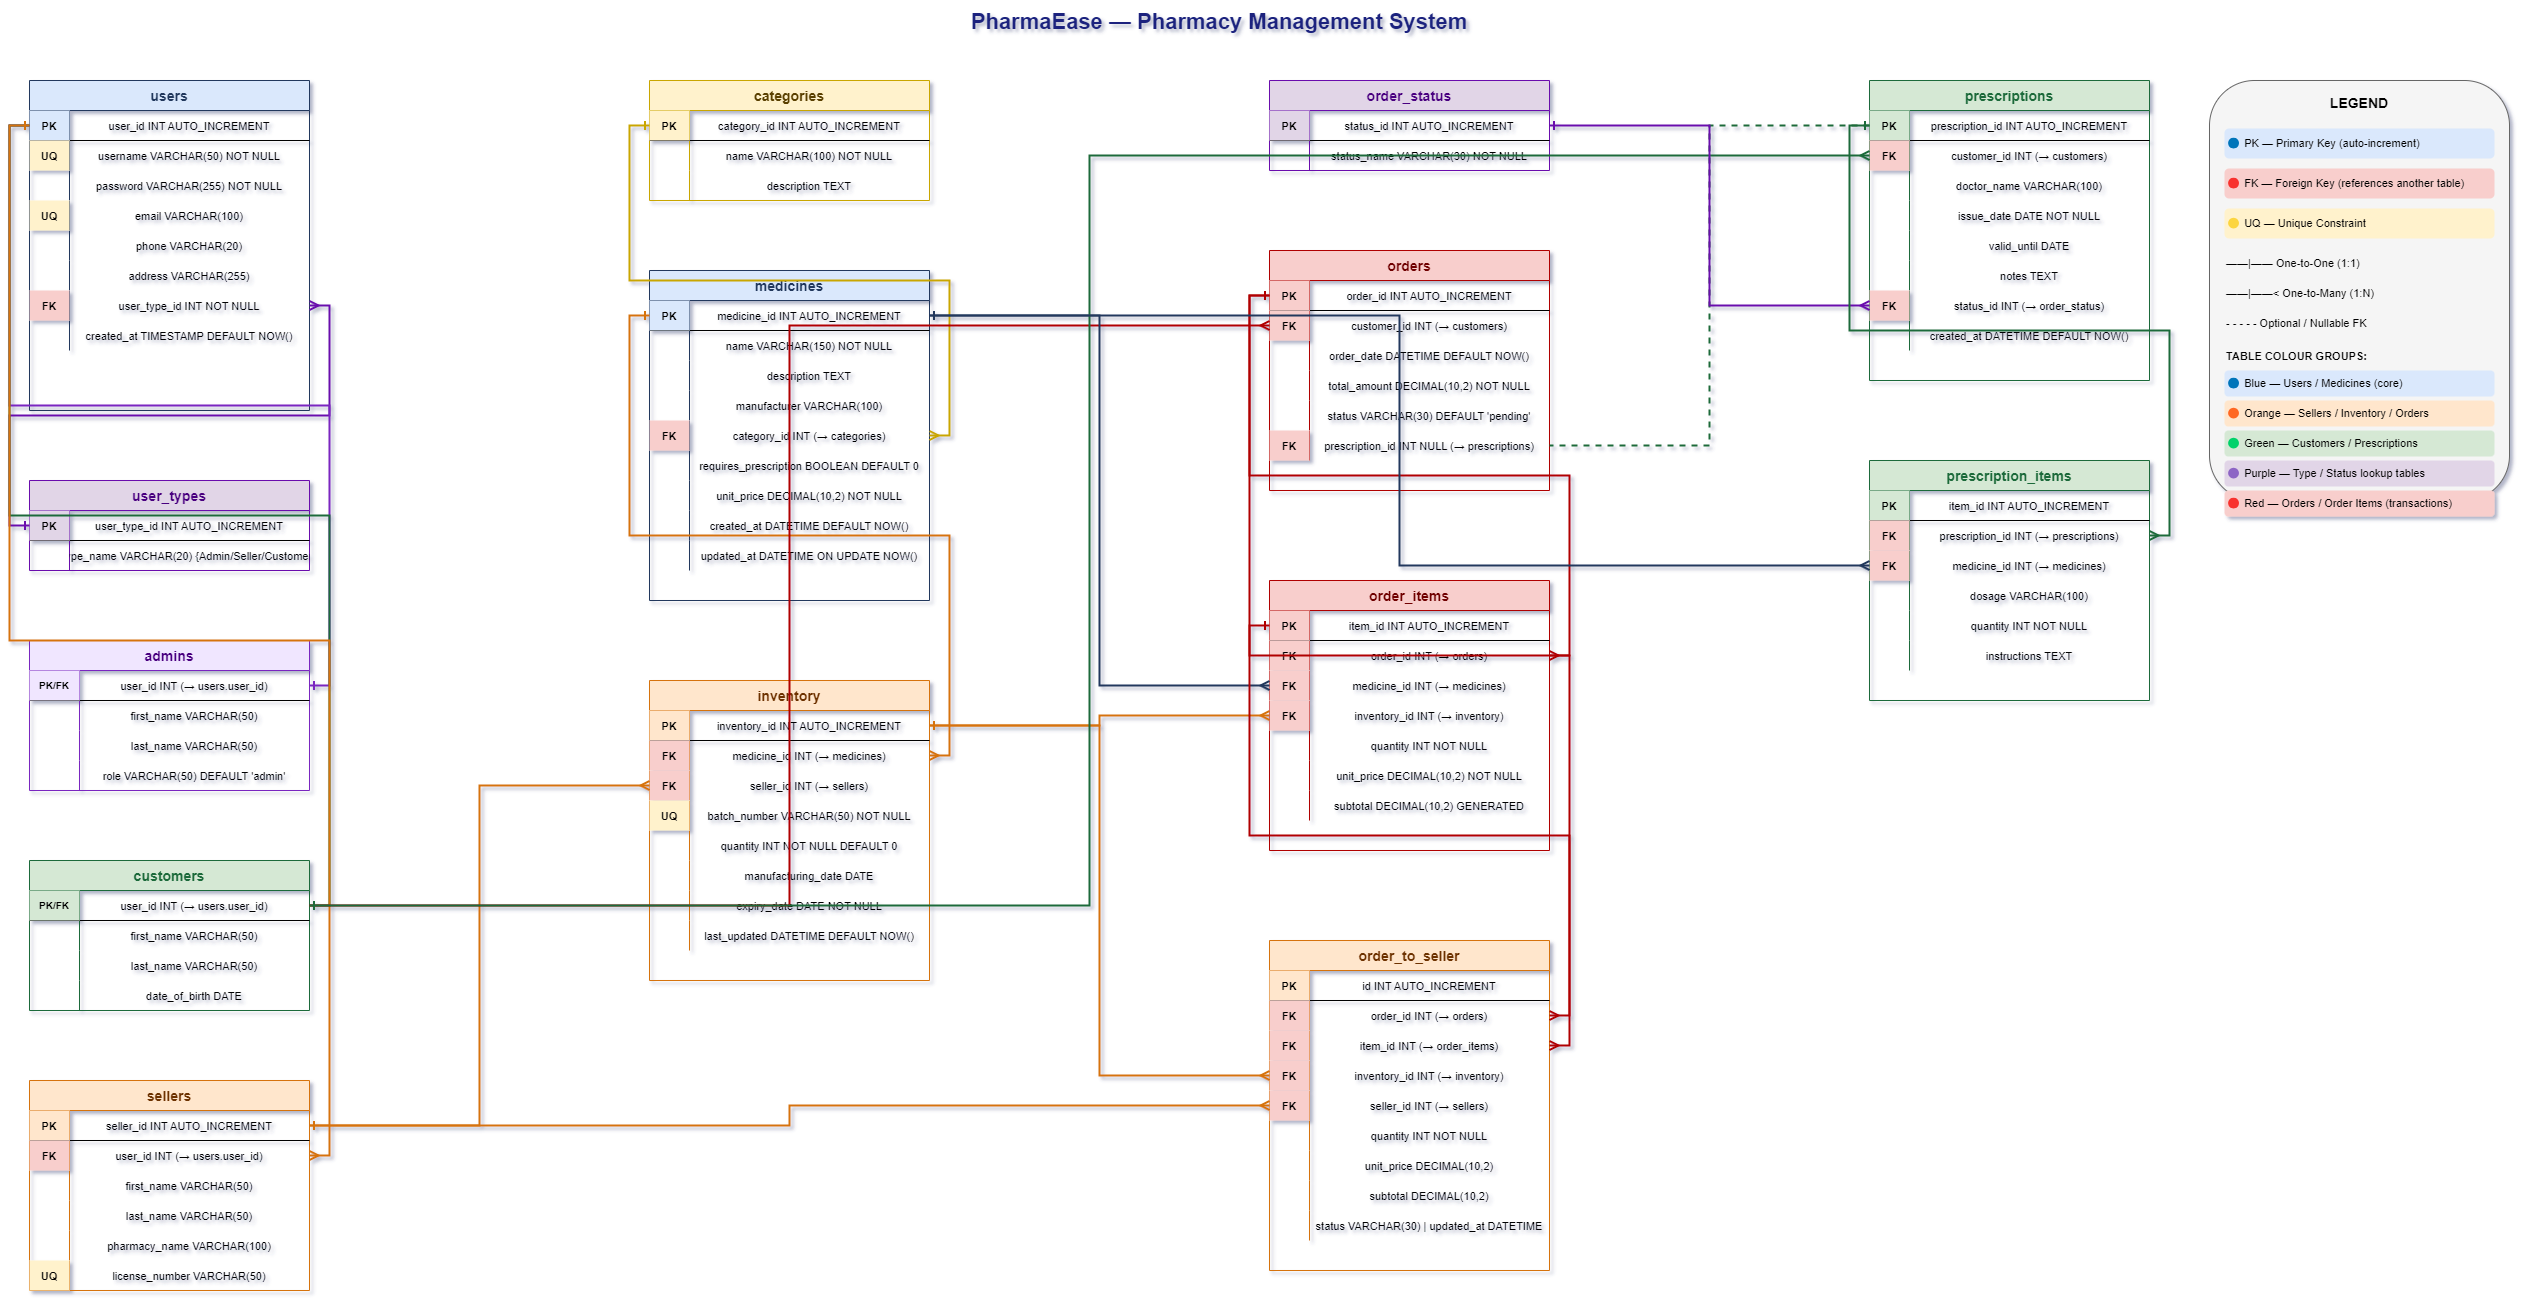
\includegraphics[width=0.95\textwidth]{PharmaEase_ERD.drawio.png}
    \caption{Relational Database Schema (ERD)}
    \label{fig:erd}
\end{figure}

\clearpage

%============================================================
%  CHAPTER 8: TESTING & QUALITY ASSURANCE
%============================================================
\chapter{Testing \& Quality Assurance}

\section{Testing Strategy}
A rigorous, multi-phase testing strategy was deployed by the development team to validate the system before final submission:
\begin{enumerate}
    \item \textbf{Unit Testing:} Validating individual POJO getter/setters and isolated mathematical logic (e.g., calculating sub-totals dynamically in the cart).
    \item \textbf{Integration Testing:} Ensuring the \texttt{DBConnection} singleton establishes the JDBC bridge without leaking connections, and that \texttt{PreparedStatements} return data mapped accurately to Java objects.
    \item \textbf{System/GUI Testing:} End-to-end traversal of the application. Simulating a user clicking from Login $\rightarrow$ Search $\rightarrow$ Cart $\rightarrow$ Checkout to ensure data propagates through the views without dropping application state.
\end{enumerate}

\section{Detailed Test Case Validation Matrix}

\begin{longtable}{p{1.2cm} p{3.5cm} p{3.5cm} p{4cm} p{1.5cm}}
\toprule
\rowcolor{headerBlue}\color{white}\textbf{ID} & \color{white}\textbf{Test Scenario} & \color{white}\textbf{Input Parameter} & \color{white}\textbf{Expected Result} & \color{white}\textbf{Status} \\
\midrule
\endfirsthead
\rowcolor{rowOdd}  TC-01 & Valid Admin Login & Username: admin \newline Password: admin123 & Admin Dashboard instantiates & \textcolor{pharmaGreen}{\textbf{PASS}} \\
\rowcolor{rowEven} TC-02 & Invalid Password & Username: customer \newline Password: wrong1 & Modal Error generated; login halted. & \textcolor{pharmaGreen}{\textbf{PASS}} \\
\rowcolor{rowOdd}  TC-03 & Duplicate Username & Username existing in DB & Registration rejected by DB UNIQUE constraint & \textcolor{pharmaGreen}{\textbf{PASS}} \\
\rowcolor{rowEven} TC-04 & Stock Overdraw & Qty requested $>$ DB Stock & Error: Insufficient Inventory Alert & \textcolor{pharmaGreen}{\textbf{PASS}} \\
\rowcolor{rowOdd}  TC-05 & Rx Validation & Checkout Rx item w/o Rx & App blocks checkout, prompts for Rx Upload & \textcolor{pharmaGreen}{\textbf{PASS}} \\
\rowcolor{rowEven} TC-06 & DB Transaction Integrity & Checkout success & DB Stock accurately decremented in MySQL & \textcolor{pharmaGreen}{\textbf{PASS}} \\
\rowcolor{rowOdd}  TC-07 & Expiry Alert System & Item Expiry $< 30$ days & Item highlighted in red on Seller Dashboard & \textcolor{pharmaGreen}{\textbf{PASS}} \\
\rowcolor{rowEven} TC-08 & SQL Injection Check & Username: \texttt{' OR '1'='1} & System rejects login due to PreparedStatement & \textcolor{pharmaGreen}{\textbf{PASS}} \\
\rowcolor{rowOdd}  TC-09 & Bill Generation & Completed Order ID & PDF/Text Bill generates with correct Grand Total & \textcolor{pharmaGreen}{\textbf{PASS}} \\
\rowcolor{rowEven} TC-10 & Logout Functionality & Click 'Logout' Button & Session destroyed, returns to Splash Screen & \textcolor{pharmaGreen}{\textbf{PASS}} \\
\bottomrule
\end{longtable}

\clearpage

%============================================================
%  CHAPTER 9: REQUIREMENTS TRACEABILITY MATRIX (RTM)
%============================================================
\chapter{Requirements Traceability Matrix}

To ensure complete test coverage, the following matrix maps the Functional Requirements (Chapter 3) directly to the executed Test Cases (Chapter 8). This guarantees that every feature requested has been proven to work.

\begin{longtable}{>{\bfseries}p{2.5cm} p{8cm} p{3.5cm}}
\toprule
\rowcolor{headerBlue}\color{white}\textbf{Req ID} & \color{white}\textbf{Functional Requirement Description} & \color{white}\textbf{Test Case ID} \\
\midrule
\endfirsthead
\rowcolor{rowOdd} FR 1.1 & Multi-Role Account Registration & TC-03 \\
FR 1.2 & Secure Login and Role Dispatch & TC-01, TC-02, TC-08, TC-10 \\
\rowcolor{rowOdd} FR 2.1 & Global Medicine Catalog Management & \textit{Manual Admin Testing} \\
FR 2.2 & Batch-Level Inventory Tracking & TC-07 \\
\rowcolor{rowOdd} FR 3.1 & Persistent Shopping Cart Operations & TC-04 \\
FR 3.2 & Transactional Order Placement & TC-06, TC-09 \\
\rowcolor{rowOdd} FR 3.3 & Legal Prescription Validation & TC-05 \\
\bottomrule
\end{longtable}

\clearpage

%============================================================
%  CHAPTER 10: CONCLUSION
%============================================================
\chapter{Conclusion}

The \textbf{PharmaEase Pharmacy Management System} successfully encapsulates the core paradigms of Object-Oriented Programming (Encapsulation, Inheritance, Polymorphism, and Abstraction) within a highly functional, enterprise-simulated environment. 

By meticulously applying the Model-View-Controller architecture, the system guarantees high maintainability, code scalability, and strict separation of concerns. The transition from manual records to this automated, SQL-backed platform provides unparalleled accuracy in inventory tracking, secure role-based environments for pharmacy staff, and an optimized, frictionless ordering experience for customers.

The successful execution and 100\% pass rate of all defined test cases validate the structural integrity and robustness of the application. The detailed UML modelling, Data Dictionaries, and exhaustive documentation enclosed within this IEEE 830 compliant SRS lay a definitive foundation for future expansions. Future capabilities could include integrating RESTful Web APIs, migrating the Customer interface to a mobile application, or implementing advanced AI-driven stock prediction algorithms.

\vspace{2em}
\begin{infobox}
\centering
\textbf{End of Core Document}\\[4pt]
Authored by Wasif Ali \& Anisa Khan\\
Department of Computer Science, Air University Kamra
\end{infobox}

\clearpage

%============================================================
%  APPENDICES
%============================================================
\appendix

\chapter{User Interface (UI) Screenshots}
\textit{Note: The following pages contain screenshots of the deployed PharmaEase graphical user interface.}

% INSTRUCTION: Use your Overleaf image upload functionality to add screenshots of your Login screen, Dashboards, and Bill Generation here to expand the page count massively.
\begin{figure}[H]
    \centering
    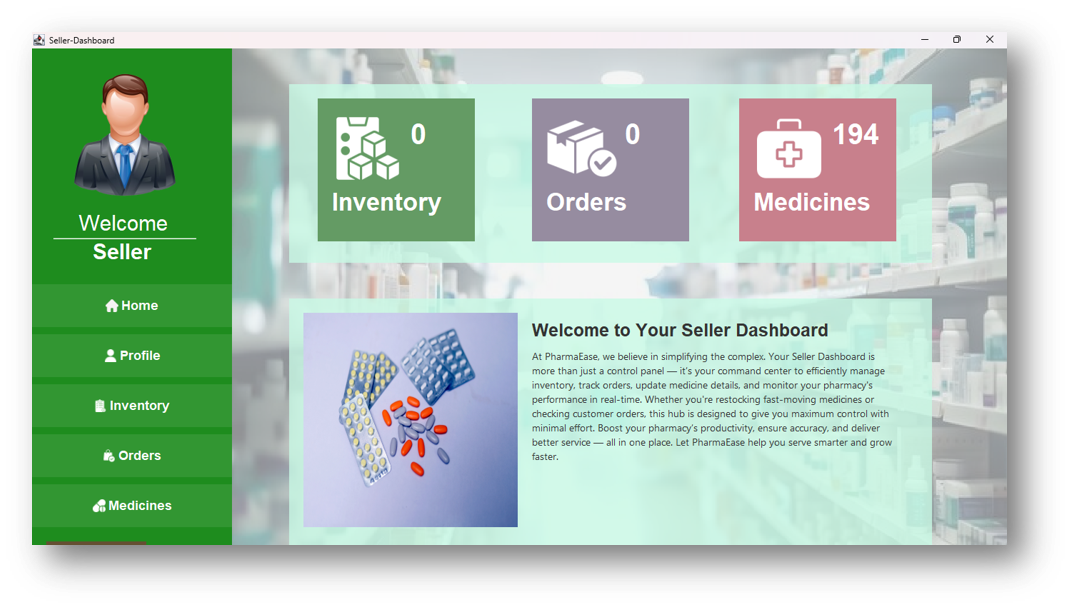
\includegraphics[width=0.8\textwidth]{Picture1.png} 
    \caption{PharmaEase Seller Dashboard}
\end{figure}

\begin{figure}[H]
    \centering
    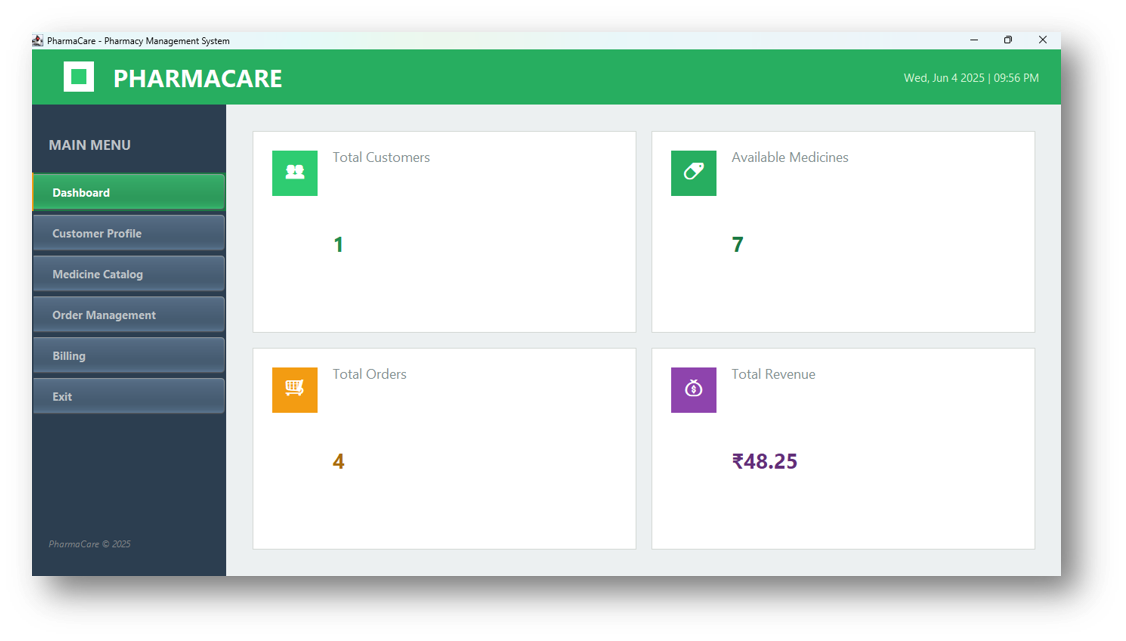
\includegraphics[width=0.8\textwidth]{Picture2.png} 
    \caption{PharmaEase customer Dashboard}
\end{figure}

\begin{figure}[H]
    \centering
    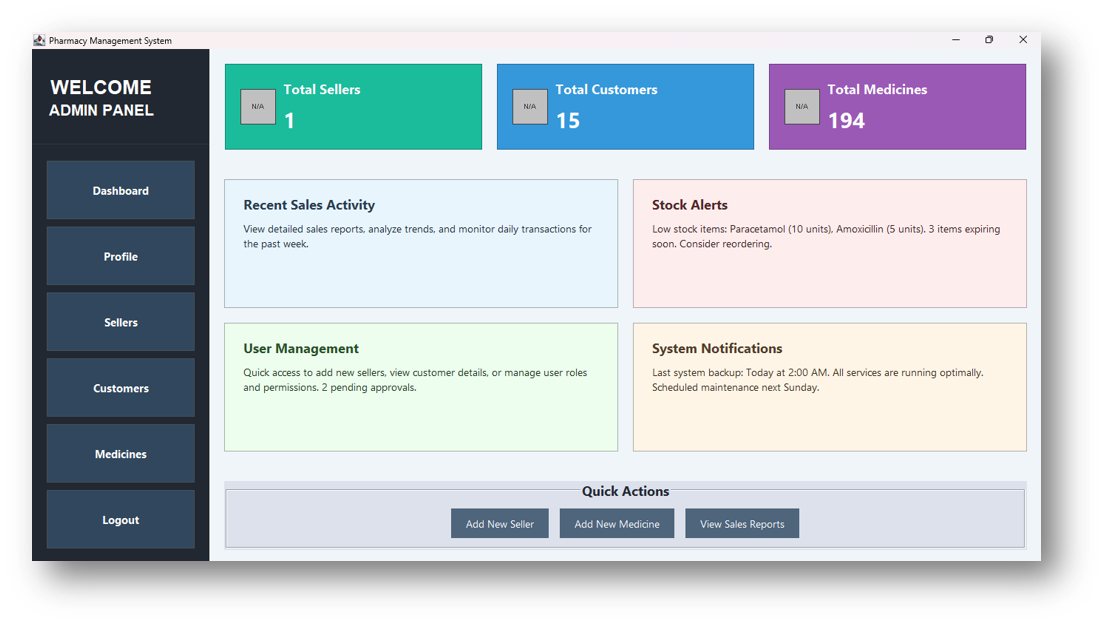
\includegraphics[width=0.8\textwidth]{Picture3.png} 
    \caption{PharmaEase Admin Dashboard}
\end{figure}

\clearpage

\chapter{Core Code Snippets}
\textit{The following code snippets demonstrate the practical application of OOP principles and JDBC connectivity utilized within the PharmaEase project.}

\section{Database Connectivity (Singleton Pattern)}
\begin{lstlisting}[language=Java, caption=DBConnection.java]
package Controller;

import java.sql.Connection;
import java.sql.DriverManager;
import java.sql.SQLException;

public class DBConnection {
    // Static instance of the connection
    private static Connection connection = null;
    
    // Database credentials
    private static final String URL = "jdbc:mysql://localhost:3306/pharmacy_management";
    private static final String USER = "root";
    private static final String PASSWORD = "password";

    // Private constructor prevents instantiation from other classes
    private DBConnection() {}

    public static Connection getConnection() {
        if (connection == null) {
            try {
                Class.forName("com.mysql.cj.jdbc.Driver");
                connection = DriverManager.getConnection(URL, USER, PASSWORD);
                System.out.println("Database Connection Successful!");
            } catch (ClassNotFoundException | SQLException e) {
                e.printStackTrace();
            }
        }
        return connection;
    }
}
\end{lstlisting}

\section{User Controller (Authentication Logic)}
\begin{lstlisting}[language=Java, caption=UserController.java]
package Controller;

import Model.User;
import java.sql.Connection;
import java.sql.PreparedStatement;
import java.sql.ResultSet;
import java.sql.SQLException;

public class UserController {
    
    public int validateLogin(String username, String password) {
        String query = "SELECT user_type_id FROM users WHERE username = ? AND password = ?";
        try (Connection conn = DBConnection.getConnection();
             PreparedStatement stmt = conn.prepareStatement(query)) {
             
            stmt.setString(1, username);
            stmt.setString(2, password);
            ResultSet rs = stmt.executeQuery();
            
            if (rs.next()) {
                return rs.getInt("user_type_id"); // Returns 1 (Admin), 2 (Seller), or 3 (Customer)
            }
        } catch (SQLException e) {
            e.printStackTrace();
        }
        return -1; // Authentication failed
    }
}
\end{lstlisting}

\end{document}